\documentclass[12pt]{report}
\usepackage{graphicx}
\usepackage{subfig}
\usepackage{listings}

\begin{document}
\lstset{language=Python}

\title{Homework 0 - Modern Analytics}
\author{Tim Delisle and Sam Raudabaugh}
\date{08/26/2015}
\maketitle


\noindent{{\large Summary}}


We investigated the relationships found in the Iris Flowers dataset in order to sanity-check our Python development environments. The attributes available for study were sepal length and width as well as petal length and width. What's interesting is to see a general pattern that could inform someone of the general size and shape of these flowers.

For one the Iris-Setosa has smaller petals (in length and width) than the other classes. It's also interesting to see that petals have relatively constant proportions (width rises with length)  for all three classes while the sepals do not.

The fact that Versicolor and Virginica are closely clustered brings up an interesting question that can't be answered by this particular data set. How are these particular flower classes related to each other genetically and in lineage? One could postulate that Vesicolor and Virginica are more closely related and bifurcated from the heritage and a more recent time.\newline

\noindent{{\large Answers to Lab Questions}}
\begin{enumerate}

\item There are 4 attributes, 3 classes and 50 instances of each class.

\item Created the vector with the following code.
\begin{lstlisting}

classes_vector = [] # Empty vector

for line in open("iris.data.txt"):
    # Ensuring that line contains the appropriate variables
    if len(line.split(",")) > 1
    	classes_vector.append(line.split(",")[4])




\end{lstlisting}

Output:

`Iris-setosa', `Iris-setosa', `Iris-setosa', `Iris-setosa', `Iris-setosa', `Iris-setosa', `Iris-setosa', `Iris-setosa', `Iris-setosa', `Iris-setosa', `Iris-setosa', `Iris-setosa', `Iris-setosa', `Iris-setosa', `Iris-setosa', `Iris-setosa', `Iris-setosa', `Iris-setosa', `Iris-setosa', `Iris-setosa', `Iris-setosa', `Iris-setosa', `Iris-setosa', `Iris-setosa', `Iris-setosa', `Iris-setosa', `Iris-setosa', `Iris-setosa', `Iris-setosa', `Iris-setosa', `Iris-setosa', `Iris-setosa', `Iris-setosa', `Iris-setosa', `Iris-setosa', `Iris-setosa', `Iris-setosa', `Iris-setosa', `Iris-setosa', `Iris-setosa', `Iris-setosa', `Iris-setosa', `Iris-setosa', `Iris-setosa', `Iris-setosa', `Iris-setosa', `Iris-setosa', `Iris-setosa', `Iris-setosa', `Iris-setosa', `Iris-versicolor', `Iris-versicolor', `Iris-versicolor', `Iris-versicolor', `Iris-versicolor', `Iris-versicolor', `Iris-versicolor', `Iris-versicolor', `Iris-versicolor', `Iris-versicolor', `Iris-versicolor', `Iris-versicolor', `Iris-versicolor', `Iris-versicolor', `Iris-versicolor', `Iris-versicolor', `Iris-versicolor', `Iris-versicolor', `Iris-versicolor', `Iris-versicolor', `Iris-versicolor', `Iris-versicolor', `Iris-versicolor', `Iris-versicolor', `Iris-versicolor', `Iris-versicolor', `Iris-versicolor', `Iris-versicolor', `Iris-versicolor', `Iris-versicolor', `Iris-versicolor', `Iris-versicolor', `Iris-versicolor', `Iris-versicolor', `Iris-versicolor', `Iris-versicolor', `Iris-versicolor', `Iris-versicolor', `Iris-versicolor', `Iris-versicolor', `Iris-versicolor', `Iris-versicolor', `Iris-versicolor', `Iris-versicolor', `Iris-versicolor', `Iris-versicolor', `Iris-versicolor', `Iris-versicolor', `Iris-versicolor', `Iris-versicolor', `Iris-virginica', `Iris-virginica', `Iris-virginica', `Iris-virginica', `Iris-virginica', `Iris-virginica', `Iris-virginica', `Iris-virginica', `Iris-virginica', `Iris-virginica', `Iris-virginica', `Iris-virginica', `Iris-virginica', `Iris-virginica', `Iris-virginica', `Iris-virginica', `Iris-virginica', `Iris-virginica', `Iris-virginica', `Iris-virginica', `Iris-virginica', `Iris-virginica', `Iris-virginica', `Iris-virginica', `Iris-virginica', `Iris-virginica', `Iris-virginica', `Iris-virginica', `Iris-virginica', `Iris-virginica', `Iris-virginica', `Iris-virginica', `Iris-virginica', `Iris-virginica', `Iris-virginica', `Iris-virginica', `Iris-virginica', `Iris-virginica', `Iris-virginica', `Iris-virginica', `Iris-virginica', `Iris-virginica', `Iris-virginica', `Iris-virginica', `Iris-virginica', `Iris-virginica', `Iris-virginica', `Iris-virginica', `Iris-virginica', `Iris-virginica'

\item Visualizations in Figure 1 on the following page

\end{enumerate}

\begin{figure}
\centering
\subfloat[sepal wid vs sepal len]{
  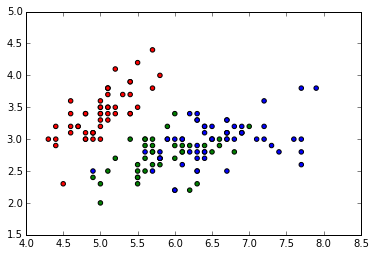
\includegraphics[width=50mm]{figures/1.png}
}
\subfloat[petal len vs sepal len]{
  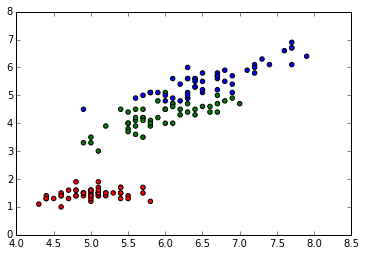
\includegraphics[width=50mm]{figures/2.png}
}
\subfloat[petal wid vs sepal len]{
  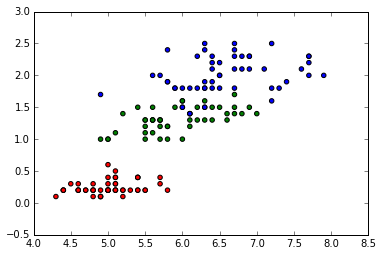
\includegraphics[width=50mm]{figures/3.png}
}
\hspace{0mm}
\subfloat[petal len vs sepal wid]{
  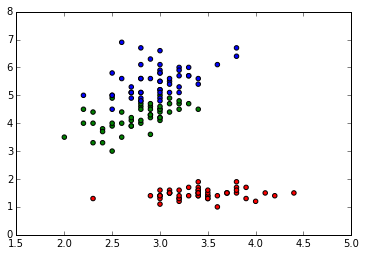
\includegraphics[width=50mm]{figures/4.png}
}
\subfloat[sepal len vs sepal wid]{
  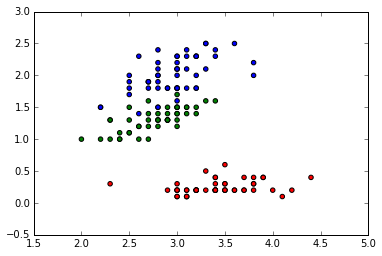
\includegraphics[width=50mm]{figures/5.png}
}
\subfloat[sepal wid vs petal len]{
  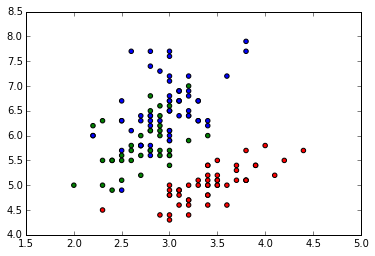
\includegraphics[width=50mm]{figures/6.png}
}
\hspace{0mm}
\subfloat[sepal wid vs petal len]{
  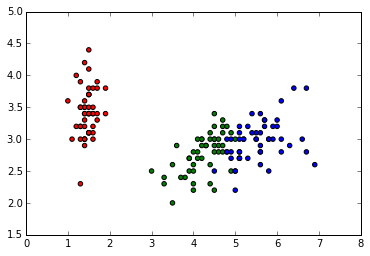
\includegraphics[width=50mm]{figures/7.png}
}
\subfloat[petal wid vs petal len]{
  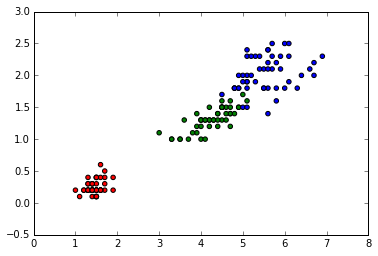
\includegraphics[width=50mm]{figures/8.png}
}
\subfloat[sepal len vs petal len]{
  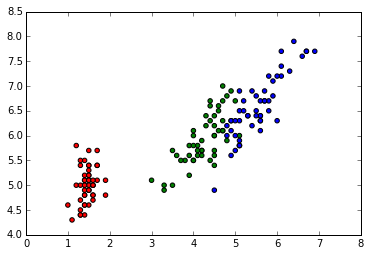
\includegraphics[width=50mm]{figures/9.png}
}
\hspace{0mm}
\subfloat[sepal wid vs petal wid]{
  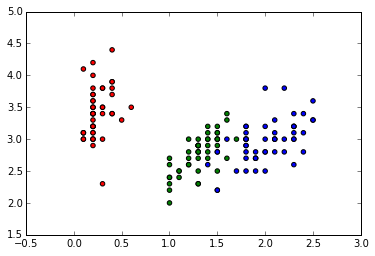
\includegraphics[width=50mm]{figures/10.png}
}
\subfloat[petal len vs petal wid]{
  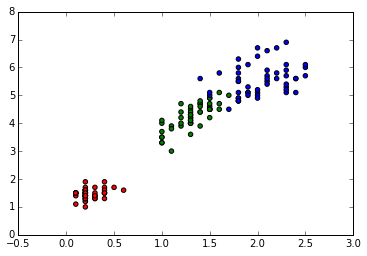
\includegraphics[width=50mm]{figures/11.png}
}
\subfloat[sepal len vs petal wid]{
  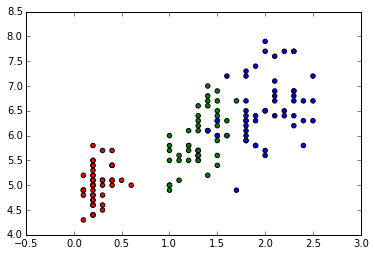
\includegraphics[width=50mm]{figures/12.png}
}
\caption{Question 3 visualizations}
\end{figure}

\end{document}
